% Thesis introduction
% Author: Tore.
%

In this chapter the background information needed in order to understand the topics of this thesis and its papers is given. First, in Section \ref{sec:gpgpu}, the history and principle of general-purpose computing on graphics processing units (\nom{GPGPU}{General-purpose computing on graphics processing units}) is reviewed, followed by an introduction to medical ultrasound imaging and adaptive beamforming in Section \ref{sec:ultrasound}. Finally, the concepts of volume rendering and ultrasound field simulations are presented in Section \ref{sec:volren} and \ref{sec:field}.

\section{General-purpose computing on graphics processing units}\label{sec:gpgpu}
In a recent essay, Herb Sutter, a leading authority on software development, reviews the current state of the software and computer industry \cite{HerbSutter}. The essay bears the name "Welcome to the Jungle" and is a sequel to the essay "The Free Lunch is Over" from 2004 \cite{HerbSuttera}. The two essays spins around the fact that manufactures of central processing units (CPUs) hit a frequency-wall in the beginning of the 21st century. Until then, all mainstream computer programs where typically running in a single thread on a single CPU \textit{processing core}, and a programmer could expect the software to annually gain performance without touching the code. This was the "free-lunch"-era as depicted in Fig.\,\ref{fig:jungle}. The increase in processing power came mostly from an ever-growing clock frequency. However, power consumption and heat generation where also growing at the same rate, until the level of cooling required finally became to much in 2004.  From that point, chip manufactures had to pursue a different direction  than just increasing the clock frequency. The immediate solution was to embed several cores in one CPU. This insured continuation of Moore's law, since the number of transistors per chip could continue to grow. For programmers, multi-core CPUs meant that computer programs now had to be multi-threaded in order to annually gain performance. It was a concurrency revolution, as Herb Sutter named it, and  the "free lunch" was over.

\begin{figure}
\centering
\includegraphics[width=0.8\textwidth]{img/free_lunsh.png}
\caption{Illustration of transitions between different eras in the computer industry. Currently there are three ongoing transitions; multi-core, heterogeneous-core and cloud-core. Image courtesy of Herb Sutter (herbsutter.com).}
\label{fig:jungle}
\end{figure}

Around the same time as CPU manufactures hit the frequency wall, people started experimenting with programmable shaders which recently had been introduced in the field of graphics programming. The graphics processing pipeline had before this been a fixed function pipeline, where e.g. geometry and textures where fed to the graphics processing unit (GPU) in one end, and where shaded a rasterized geometry was outputted in the other. What programmable shaders  introduced was the ability to replace some steps in the fixed-function pipeline with custom computations. This made it possible to utilize the GPU for other tasks than just rendering graphics \cite{Seland2007}. The rationale behind this exploration was that GPUs were already highly available in consumer PCs, and hidden behind its graphics interface were processing powers an order of magnitude larger than what the CPU could provide (Fig.\,\ref{fig:cpu_vs_gpu}). Actually, at the time when CPU manufacturers hit the frequency wall the GPU had already gone multi-core, first of all driven by an ever-increasing demand for more realistic computer games. Secondly, the rendering pipeline exhibits minimal execution path branching, and data are typically used once. Designers of GPUs could therefore skip advance feature, found in most CPUs, like branch prediction and different levels of data caching. These measures reduced the silicon footprint of each core and made it possible to add multiple cores to one GPU before CPU designers where able to do the same. Today, even if more advanced caching has been added to GPUs, this is still the main reason why GPUs have higher peak performance than CPUs (Fig.\,\ref{fig:cpu_vs_gpu}). Another reason is the inherent parallel nature of the rendering problem. When geometry is shaded, projected and rasterized the same instruction is typically needed for a lot of data at the same time. This makes a special kind of instruction, known as Single Instruction Multiple Data (\nom{SIMD}{Single instruction multiple data (instruction type)}) \cite{Flynn1966}, especially suited for this kind of problem. The differences between how SIMD instructions are utilized in modern CPUs and GPUs are discussed in Section \ref{sec:cpu_vs_gpu}.

For the first adopters of general-purpose computing on GPUs (GPGPU) it soon became evident that offloading all types of computations to the GPU was not always a good idea. In most cases it is important to balance the load equally between the CPU and GPU to obtain their combined computationally power. Balancing typically means that highly parallel and computationally intense tasks should be offloaded to the GPU and serialized and memory intensive work should stay on the CPU. This paradigm of utilizing specialized cores for solving specific problems is today known as \textit{heterogeneous computing}. The specialized core can be a GPU or e.g. a field-programmable gate array (\nom{FPGA}{Field-programmable gate array}). A recent trend is that specialized accelerator cores are embedded onto the CPU. This heterogeneous processors is often referred to as an accelerated processing unit (\nom{APU}{Accelerated processing unit}). The last three generations of CPUs from Intel have all had on-chip integrated graphics, hence they can be classified as APUs. An on-chip GPU is less powerful than a high-performance discrete GPU, but valuable time is saved by not having to send data across the PCI Express bus, which connects the different parts of a computer to the motherboard. This is the reason why one of the first rules of GPGPU (with discrete GPUs) is to minimize CPU-to-GPU memory transfers. 

The final transition currently taking place in the computer industry is the introduction of cloud computing, where compute power is provided as a web service and automatically scales on demand. Together, multi-core, heterogeneous cores, and cloud cores forms the "jungle" that today's software engineers have to tackle (Fig.\,\ref{fig:jungle}). In this thesis we focus on heterogeneous computing with one multi-core CPU and a discrete high performance GPU, a cheap and high performance system which is likely to be the specification of current and future ultrasound imaging system.

\subsection{Comparing CPU and GPU performance}\label{sec:cpu_vs_gpu}
The CPU is design to be the main control unit of a computer, it is therefore good at general processing. The GPU, on the other hand, has a history of processing graphics which involves heavy vector arithmetic. Even though they started out as very different processors, modern CPUs are including more and more GPU-like features, and GPUs are adding CPU features. In this section we will see what these similarities are and why there is still a big difference in peak performance between a CPU and a GPU.

\begin{figure}
\centering
\includegraphics[width=0.8\textwidth]{img/CPU-GPU.pdf}
\caption{Schematic overview of CPU (Intel Haswell) and GPU (Nvidia Kepler) architecture. Note how more space is dedicated to compute cores on a GPU, and how more space is dedicated to control and caching on a CPU.}
\label{fig:cpu_gpu}
\end{figure}

In Section \ref{sec:gpgpu} we introduced a special type of instructions, namely SIMD instructions, which are designed to execute a single instruction across multiple data element in one clock cycle. At the end of the 20th century, Intel introduced a SIMD instruction set for their Pentium III processor called the Streaming SIMD Extensions (\nom{SSE}{Streaming SIMD extensions (instruction set)}), which has seen several updates since. The first SEE instructions set had 128 bit long registers which meant that four, 32 bit, floating point values could be processed per clock cycle\footnote{For simplicity we will assume that the whole register is processed in one clock cycle even if the actual implementation might distributes one instruction for the register across multiple cycles.}. Updates of the SSE instruction set have added new instructions and longer registers (SSE2, SSE3, SSE4, \nom{AVX}{Advanced vector extensions (instruction set)}, AVX2, and AVX-512). The newly introduced extensions, AVX and AVX2, adds 256 bit long registers and fused multiply-accumulate instructions (\nom{FMA}{Fused multiply-accumulate (instruction)})  which means that sixteen 32 bit floating point operations can be performed per clock cycle per core. A new extension, AVX-512, extends the registers to 512 bit and is found in the Intel accelerator board  Xeon Phi and might show up in the next generation of CPUs from Intel. The latest CPU architecture from Intel, the Haswell architecture, has two processing ports per core supporting FMA-AVX2 instructions, and is therefore capable of performing 32, 32 bit, floating point operations per clock cycle per core (Fig.\,\ref{fig:cpu_gpu}). For an eight core\footnote{An 8-core Haswell CPU is scheduled to launch during 2014.} CPU with a clock frequency of 3.8 GHz this sums to 
\begin{equation}
32*8*3.8 = 972.8\,\text{GFLOPS},
\end{equation}
hence a theoretical peak performance of close to one tera single precision floating point operations per second (TFLOPS). This is the same number as visualized in Fig\,\ref{fig:cpu_vs_gpu} for the Haswell architecture (Single precision). In addition, the most powerful integrated GPU found on Haswell CPUs, the HD 5200, has 40 execution units capable of processing sixteen, 32 bit, floating points at 1.3 GHz. This adds
\begin{equation}
16*40*1.3 = 832\,\text{GFLOPS}
\end{equation}
in extra processing power to the APU.

Modern GPUs can also be interpreted as a unit consisting of multiple SIMD cores (Fig.\,\ref{fig:cpu_gpu}). The recent Kepler architecture by Nvidia have up to 15 SIMD units capable of processing 192, 32 bit, floating point values per clock cycle at 745 MHz\footnote{Nvidia typically refers to a core as a unit capable of performing a FMA instruction on one single precision floating point value. Hence, in Nvidia's world, Kepler has $15*192=2880$ cores.}. These GPUs are also capable of performing FMA instructions, effectively doubling the number of theoretical FLOPS. The theoretical peak single precision FLOPS for this architecture is by that found to be 
\begin{equation}
15*192*2*745 = 4291\,\text{GFLOPS}.
\end{equation} 
Each SIMD core also comprise 16 special function units (\nom{SFU}{Special function unit (sin, exp, sqrt, ect.)}) which add close to 1 TFLOPS in additional computational power. This adds up to a total of five TFLOPS as shown in Fig.\,\ref{fig:cpu_vs_gpu} for the GeForce GTX 780 TI GPU. From Fig.\,\ref{fig:cpu_gpu} we see how the high number of SIMD cores found on GPUs and their larger width, compared with the SIMD cores on CPUs, results in five times the computational performance of a high-end CPU (without the integrated GPU). 

Note that the derived numbers are strictly theoretical and that actual throughput is highly algorithm dependent. Nevertheless, in theory, the benefit of GPU computing over CPU computing is currently a factor of five in raw computationally power. A claimed speed-up of several order of magnitude is typically a result of comparing a non-optimized CPU implementation with an optimized GPU implementation or by comparing uneven hardware \cite{Lee2010, Kothapalli2013}. In this section we have focused on CPUs from Intel and GPUs from Nvidia, however, CPUs and GPUs from AMD have similar specifications and differences in theoretical peak performance. 

\begin{figure}
\centering
\includegraphics[width=\textwidth]{img/cpu_vs_gpu.pdf}
\caption{Development in theoretical peak throughput, single precision (SP) and double precision (DP), the last decade for Intel CPUs and Nvidia GPUs.}
\label{fig:cpu_vs_gpu}
\end{figure}

\subsection{Programming a GPU}
Early GPGPU programming required expert knowledge about computer graphics and the remaining fixed functions in the graphics pipeline. When GPGPU gained interest and the GPU was used to compute problems that did not involve graphics, it quickly became evident that new programing languages where needed.  One of the first GPGPU oriented languages for the GPU was the Brook language by Buck \textit{et al.} \cite{Buck2004}. Buck later joined Nvidia where he led the work on \nom{CUDA}{Compute unified device architecture (GPGPU framework)}, a GPGPU language and framework by Nvidia for Nvidia GPUs only. The first version of CUDA was released in 2007. The following year, Apple launched a GPGPU framework known as \nom{OpenCL}{Open Compute Language (GPGPU framework)}, a standard which are maintained by the Khronos Group. These two frameworks are still today the main programming frameworks for GPGPU. Where CUDA only runs on Nvidia GPUs, OpenCL can now run on GPUs from both Nvidia and AMD, CPUs from both Intel and AMD, FPGAs from Altera, and mobile processors from \nom{ARM}{Designer of mobile chip architectures}.

\begin{figure}
\centering
\subfigure[Kernel]{
	\includegraphics[width=0.5\textwidth]{img/kernel.pdf}\label{fig:gpu_kernel}
}
\subfigure[Threads, blocks and grid]{
	\includegraphics[width=0.4\textwidth]{img/cuda_threads.png}\label{fig:gpu_grid}
}
\caption{The figure depicts how GPU threads are grouped into blocks and arranged in a grid. One thread runs a copy of a kernel function. In this example the kernel function performs an in-place element-wise matrix square.}
\label{fig:gpu_grid_kernel}
\end{figure}

Both CUDA and OpenCL is centered around a kernel function which are executed by a large group of threads. The kernel function, for both CUDA and OpenCL, has a C-like syntax with some additional specifiers. An example of a CUDA kernel is depicted in Fig.\,\ref{fig:gpu_kernel}. The \texttt{\_\_global\_\_} specifier tells the CUDA compiler that this function is a kernel function, and in CUDA, this kernel function is launched by using a CUDA specific syntax:
\begin{align*}
\texttt{square<<<grid, block>>>(a, N)},
\end{align*}
where \texttt{grid} and \texttt{block} is 3-component vectors specifying grid and block size in "xyz" as depicted in Fig.\,\ref{fig:gpu_grid}, \texttt{a} is a pointer to a memory buffer located on the GPU, and \texttt{N}$*$\texttt{N} is the size of the buffer \texttt{a}. 

When the kernel is launched, a copy of it is scheduled for each thread in each block, and each kernel instance gets as input its location in the compute grid (\texttt{blockIdx} and \texttt{threadIdx}) together with the grid size (\texttt{gridDim} and \texttt{blockDim}). This information is then typically used to calculate which memory elements to gather from global memory, in this case the elements in \texttt{a}. %Behind the scene, thread blocks are divided into smaller sets of threads called a warp (or wavefront in OpenCL). 
When a kernel is executed, multiple thread blocks are scheduled to each SIMD core where they stay until all instructions in the kernel is finished for all threads in the block. Thus,  in order to formulate a given problem as a kernel function the global memory input to each thread must not depend on the output from other blocks, hence, it must be possible for the GPU to schedule blocks in any order. 

As we see, a thread has a different conceptual meaning on a GPU than on a CPU.  Where a CPU is said to execute threads which can perform SIMD instructions, a thread on a GPU can be interpreted as unit capable of processing one data element in the SIMD instruction. This is why GPU threads are said to be light weighted. This conceptual difference also means that there is an inherent focus on breaking algorithms down and into SIMD instructions when programing for the GPU. This often leads to a highly optimized parallel implementation on the GPU and not on the CPU. Threads, or SIMD instructions, is just how one program for the GPU, there is no other way of doing it.

It is important to understand that not all algorithms will benefit from wider SIMD registers. As the width increase the only algorithms that will benefit is those who can be divided into enough concurrent fine granular parts. Also, to achieve peak performance, the implementation must perform one FMA operation on each core per clock cycle and all memory latency must be hidden by issuing instructions. All of this is something which is impossible to achieve in real life applications. One will always end up with a throughput which is a fraction of the peak throughput.

The code in Fig.\,\ref{fig:gpu_grid} is of course a minimal example of GPU programing. A full example will involve several lines of C++ code transferring data to and from the GPU, and the kernel could include manual administration of the L1 cache (shared memory), and intra-block thread barriers. This is some of the reasons why writing a high performance GPU kernel is often found to be a complex and time consuming task. Because of the major overhead involved with writing GPU code we will, in the future, probably see a lot of work aimed at reducing it.  A recent development is the introduction of C++ AMP which enables developers to write accelerated code (e.g. by a GPU) in plain C++. Hopefully, in near future, GPU programming will be a job for compilers, and direct fiddling with GPU kernels should only be needed if maximum throughput is absolutely needed. This is similar to how SIMD instructions are handled in CPU-code today. Most of the time developers will rely on the CPU compilers to analyze the code and auto-apply SIMD instruction whenever it is possible. However, when maximum throughput is needed, developers with deep knowledge of the algorithm are often able to make faster code by manually writing SIMD instruction code. The relevance of auto-applied GPU instructions by compilers will also increase due to the recent embedding of GPUs on the same chip as the CPU. Soon, when writing code, we will probably talk about coding a heterogeneous collection of cores where operations are automatically offloaded to the right core (e.g. a GPU) by the compiler.

\section {Medical ultrasound imaging}\label{sec:ultrasound}
Ultrasound imaging encompasses technology which generates images based on sound whose frequencies we can not hear. For medical ultrasound imaging frequencies between 2 MHz and 10 MHz are typically used. Which frequency to select depends on how deep into the body we want to image, this because human tissue exhibits frequency dependent attenuation. Frequency dependent attenuation is the reason why a frequency around 3 MHz is used for fetal and cardiac imaging and a frequency around 7 MHz is used for more shallow imaging (e.g. vascular imaging). 

Medical ultrasound imaging is considered to be a low-risk tool for non-invasive investigation. There are no gamma rays or high intensity magnetic fields involved, just sound pressure below well controlled limits. It is also far less costly than other imaging modalities and offers real-time inspection of the human body.  Ultrasound imaging is well know for its use in fetal imaging during pregnancy, however, in this thesis we will focus on a different modality, namely cardiac ultrasound imaging. An illustration of the human heart is therefore included in Fig.\,\ref{fig:human_heart}. Throughout the thesis we will refer to some of the parts shown in Fig.\,\ref{fig:human_heart}. Especially note the four chambers of the heart, the left and right atrium, and the left and right ventricle. The tissue separating the left and right ventricle is know as the inter-ventricular septum. The left side is the strongest and hardest working part of the heart, and it is responsible of pumping blood out to the whole body through the aortic valve. When blood flows out the aorta it is important that the mitral valve, that separates the left atrium and ventricle, is closed and does not leak. The left ventricle and the mitral valve therefore receives special attention during cardiac ultrasound examinations. When visualizing 3D ultrasound images in \textbf{Paper IV} we will have a strong focus on visibility of cardiac tissue, thus note for later that the endocardium refers to the innermost layer of the cardiac muscle.

\begin{figure}
\centering
\subfigure{
	\includegraphics[width=0.47\textwidth]{img/Diagram_of_the_human_heart.png}
}
\subfigure{
	\includegraphics[width=0.47\textwidth]{img/HeartWall.png}
}
\caption{Overview of the human heart. Illustrations from wikipedia.org.}
\label{fig:human_heart}
\end{figure}

To generate the ultrasonic frequencies used for imaging a piezoelectric ceramic is used. A piezoelectric material is special in that way that ultrasound vibrations are generated when voltage is applied and \textit{vice versa}. It can therefore be used to both send and receive ultrasound signals, like a combined microphone and speaker. Piezoelectric elements organized in an array, is referred to as an ultrasound \textit{probe}, and a special probe is typically designed for each medical imaging modality. For cardiac ultrasound imaging the probe must not only be designed for a certain frequency range, its footprint also needs to be smaller than the intercostal window in order to avoid shadowing by ribs. A line in an ultrasound image is generated by firing a ultrasound pulse into the body and sample the received echo. This amplitude trace is known as an A-mode image. 

If the width of a piezoelectric element is less than the wavelength of the transmitted signal the element is said to be \textit{omnidirectional}, hence energy is distributed or sensed equally in all directions. When multiple omnidirectional elements are arranged in a linear array the transmitted pulse will get shaped into a beam\footnote{A beam refers to the pulse in space integrated across time.} of ultrasound by diffraction as the size of the array  (the \textit{aperture}) grows. The 3 dB angular width of this beam, and also the angular resolution of the array, is given by \cite{AngelUltrasound}:
\begin{align}\label{eq:res}
\delta\theta_a = \frac{\lambda}{D} = \frac{c}{fD},
\end{align}
\nomi{$\delta\theta_a$}{Angular resolution of an aperture}where \nom{$\lambda$}{Wavelength} and \nom{$f$}{Frequency} is the ultrasound wavelength and frequency respectively, $c$ is the speed of sound, and \nom{$D$}{Aperture size} is the aperture width. With an average speed-of-sound in human tissue of $1540\frac{\text{m}}{\text{s}}$, the angular resolution or opening angle of a 2 cm cardiac probe operating at 3 MHz is around 1.5\degree, which at 8 cm range gives a lateral resolution of around 2 mm. The axial resolution is inverse proportional to the pulse length, and is typically better than the lateral resolution.

\begin{figure}
\centering
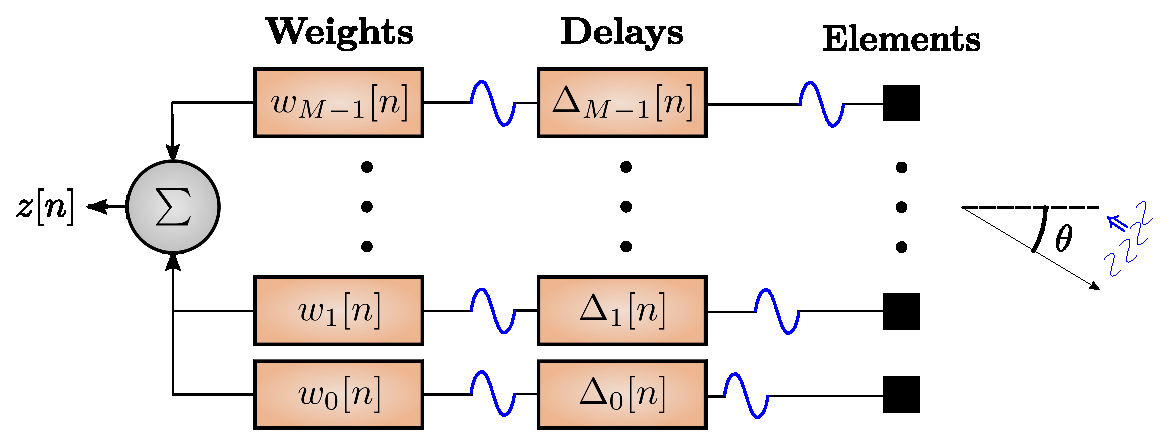
\includegraphics[width=0.8\textwidth]{img/beamforming_das.eps}
\caption{Delay-and-sum array beamforming.}
\label{fig:das}
\end{figure}

If time delays are applied on the signal sent to the different elements it is possible to steer and focus the ultrasound beam in space (Fig.\,\ref{fig:das}). This technique is known as \textit{beamforming}, and for ultrasound imaging it is traditionally applied both when transmitting and receiving ultrasound pulses. For medical ultrasound imaging there are two main types of ultrasound probes, linear and phased probes \cite{AngelUltrasound}. A cardiac probe is a phased probe, which means that the image is constructed from beams, or A-mode images, which are gradually steered from $-\theta/2$ to $\theta/2$ radians, resulting in an imaging sector which are $\theta$ radians wide. This kind of image, where A-mode images are acquired from multiple spatial locations in the $xz$-plane, is known as a B-mode image (B for brightness). If A-mode images are acquired from the $yz$-plane as well we get what is known as a volumetric B-mode or 3D ultrasound image. A probe for 3D imaging has several thousand elements arranged as a matrix. In this thesis we will focus on linear arrays for 2D imaging when the topic is adaptive beamforming, and 3D imaging when the topic is adaptive visualization.

If \nom{$M$}{Number of array elements} is the number of elements in the array, and \nom{$\Delta_m$}{Per-element focusing and steering delays} is the per-element focusing and steering delay, the standard form of beamforming used on receive, known as \textit{delay-and-sum}, is given as:
\begin{align}\label{eq:das}
z[n] = \sum_{m = 0}^{M-1}w_m^*x_m[n - \Delta_m[n]] = \vec{w}^H\vec{x}[n],
\end{align}
where \nom{$\vec{w}$}{Array weight vector (apodization)} is know as the array \textit{weight vector} or \textit{apodization}, and $z[n]$ is the output A-mode image in the direction given by $\Delta_m[n]$.  A schematic overview of delay-and-sum array beamforming is depicted in Fig.\,\ref{fig:das}. If $p_o$ is the phase center of our array and $p$ is the point where we want to steer and focus the ultrasound beam, we have to use the following delays:
\begin{align}
\Delta_m[n] =\frac{|p_o+p| - |p_m+p|}{c},
\end{align}
where \nom{$c$}{Speed of sound} is the speed of sound in human tissue, and $p_m$ is the position of the m'th element. On transmit the inverse set of delays has to be used. Also note that on transmit we have to decide where to steer and focus prior to transmitting a pulse, transmit delays therefore do not vary within an A-mode image.

When generating a B-mode image we have to insure that the spatial and temporal sampling are sufficient. We have already seen that the lateral resolution of an ultrasound probe is given by (\ref{eq:res}).  Hergum \textit{et al.} \cite{Hergum2009} have further shown that the lateral frequency support for a system which both emit and receive energy is governed by the sum of the transmit (\nom{tx}{Transmit}) and receive (\nom{rx}{Receive}) aperture. The lateral resolution of what is known as an active imaging system is found to be
\begin{align}
\delta\theta = \frac{\lambda}{D_{tx} + D_{rx}}.
\end{align}
\nomi{$\delta\theta$}{Angular resolution of a two-way imaging system}\nomi{$D_{tx}$}{Aperture size on transmit}\nomi{$D_{rx}$}{Aperture size on receive}Then, in order to properly sample an imaging sector of $\theta$ radians we have to acquire 
\begin{align}
N_\theta = \frac{\theta}{\delta\theta}
\end{align}
\nomi{$N_\theta$}{Number of lines required for proper sampling of an imaging sector}A-mode images uniformly distributed across the sector. If \nom{$r$}{Imaging range.} is the maximum range we want to image we get an imaging frame rate of
\begin{align}
f_{\text{FPS}} = \frac{c}{2rN_\theta}
\end{align} 
frames per second (\nom{FPS}{Frames per second}). With our 2 cm cardiac probe from the earlier example we get a frame rate of around $55$ FPS when imaging a 70\degree{} sector with $r=15$ cm.

The required axial sampling is dictated by the transmit frequency and the frequency bandwidth of the probe. From Fourier theory we know that a short impulse consist of many frequency components. A short ultrasound pulse, which would yield high axial resolution, therefore requires a large frequency bandwidth. A ultrasound probe has normally a relative bandwidth between 50 and 100 \%. This corresponds to transmitting a pulse which are between 2 and 1 oscillation long. In the front-end of an ultrasound imaging system a high sampling frequency is typically used (e.g. 40 MHz). However, the ultrasound signal is band limited, and the data rate can therefore be reduced in a process known as \textit{\nom{IQ}{In-phase quadrature (ultrasound data format).} demodulation}. In this process the axial sampling rate is reduced to the bandwidth of the imaging system in the following three steps: demodulation with a complex exponential, low-pass filtering, and decimation. The number of samples in one A-mode image is after this process given by:
\begin{align}
N = \frac{2r}{c}B,
\end{align}
\nomi{$N$}{Number of samples in range}where \nom{$B$}{Frequency bandwidth} is the bandwidth, $B = B_wf_c$ (where \nom{$B_w$}{Relative bandwidth} is the relative bandwidth and \nom{$f_c$}{Center frequency of ultrasound pulse} is the center frequency of the transmitted pulse). The total number of samples in an B-mode image is then 
\begin{align}
N_{\text{B-mode}} = N_\theta N.
\end{align}
If our cardiac probe has a relative bandwidth of $80$ \% we have to process almost $50000$ $M$-long vectors of element data every $1/55$ second. The formula for the number of FLOPS required for real-time DAS beamforming of cardiac ultrasound is then given as:
\begin{align}
\text{FLOPS}_{\text{DAS}} = MN_{\text{B-mode}}f_{\text{FPS}} = MB_wf_c
\end{align}
If our cardiac probe has $M=128$ elements, DAS beamforming requires a processing throughput of around $300$ MFLOPS. Hence, far below the peak processing throughput of modern GPUs and CPUs. The main challange with DAS beamforming is the amount of data that has to be moved. If one element sample is two bytes long, for our example, around 600 MB has to be moved on to the GPU every second. This is however less than the maximum bandwidth of PCI Express 2.0 (8 GB/s), even if the relative bandwidth, transmit frequency and number of array elements are increased with a total factor of 10.

%Time v.s. phase delays. It is well described in the paper using phase delays.

\subsection{GPUs in medical ultrasound imaging}
Ultrasound imaging systems generates an incredible amount of data. A modern system capable of 3D imaging will generate several tera bytes of data in the front end of the system during a clinical scan. The data rate from a 2D scan is "only" in order giga bytes per second. To handle these amount of data, ultrasound imaging systems have relied heavily on application-specific integrated circuits (\nom{ASIC}{Application-specific integrated circuit}) for all steps in the processing pipeline. However, as the computationally power of CPUs and GPUs have increased, ASICs, e.g. for converting data from a polar to a Cartesian grid (known as scan conversion), have gradually been converted into software \cite{Guracar2013}. One of  the last remaining ASICs is the beamformer, whose job is to steer and focus the ultrasound beam in space. This operation involves a reduction of the data rate with a factor equal to the number of elements in the ultrasound probe. The input data rate is therefor very high. Nevertheless, real-time beamforming has recently been achieved on a GPU \cite{Song2012}, and a French company (SuperSonic Imagine) are utilizing GPUs in their plane wave beamforming algorithm \cite{Tanter2014}. Beamforming is therefore finally moving into software too. The largest players in the medical ultrasound business, General Electric and Philips, are also well aware of where the trend is going \cite{Thomenius2012} \cite{Metz2011}. Software beamforming opens up new possibilities for advanced processing of ultrasound data. One example is Capon beamforming which is explored in this thesis (\textbf{Paper\,I} and \textbf{II}). The increased computational power introduced by GPUs makes it also possible to include advanced 3D visualization as presented in \cite{solteszova2010multidirectional}, \textbf{Paper\,IV}, and \textbf{IX}.

\subsection{Adaptive beamforming}\label{sec:adaptbf}
Adaptive beamforming has several meanings in the medical ultrasound literature. It can for instance refer to aberration correction which is the task of applying time delays to compensate for the distortion introduced by fatty layers in the human body. However, in this thesis adaptive beamforming will refer to data-dependent apodization (or weighting) derived from a given optimization criterion. The optimization criterion which we focus on in this thesis is the minimum variance distortionless response criterion, which is also known as Capon's method \cite{Capon1969}. A beamformer which uses weights derived using Capon's method will in this thesis mainly be referred to as the \textit{Capon beamformer}. However, it is also known as the minimum variance  (\nom{MV}{Minimum variance beamformer}) beamformer or the minimum variance distortionless respons beamformer (\nom{MVDR}{Minimum variance distortionless respons beamformer (Capon)}).

\begin{figure}[t!]
\subfigure[Uniform weights]{
	\includegraphics[width=0.47\textwidth]{img/scenario_das_resp2.png}\label{fig:das_weights}
}
\subfigure[Capon weights]{
	\includegraphics[width=0.47\textwidth]{img/scenario_mv_resp2.png}\label{fig:capon_weights}
}
\caption{Examples of array beampatterns where the array weights are either uniform (a) or derived using Capon's method (b). An interfering source is located at 20\degree. Notice the reduced sidelobe level for the Capon beampattern in the direction of the interfering source. Image courtesy of Jo Inge Buskenes.}
\label{fig:weights}
\end{figure}

The Capon beamformer produces a weight vector, as introduced in (\ref{eq:das}), based on the impinging signal and an optimization criterion. The problem is as follow \cite{Capon1969}:
\begin{align}
&\min_{\vec{w}} E\{|z[n]|^2\} \rightarrow \min_{\vec{w}} \vec{w}^H \mat{\hat{R}} \vec{w} \label{eq:capon_optimization_criteria} \\
&\text{subjected to } \vec{w}^H\vec{a} = 1,
\end{align}
where \nom{$\mat{\hat{R}}$}{Sample covariance matrix (with regularization)} is a sample covariance matrix. Hence, the resulting weight vector minimizes the output power (the criterion) while maintaining unit gain in the steering direction $\vec{a}$ (distortionless response). The benefit of adaptive beamforming is clearly seen from Fig\,\ref{fig:weights} which shows a sensitivity map (an \textit{array beampattern}) for DAS beamforming with uniform weights and the Capon beamformer. In this simulated case an interfering source is located at 20\degree{} which for the DAS beamformer with uniform weights (\ref{fig:das_weights}) will leak into the beamformer output with its power attenuated with around $13$ dB. Since the Capon weights are data-dependent the method "knows" where the interfering source is located and is able to position a zero in the direction of it. Hence, the interfering source will be highly attenuated independent of its direction. Another interesting case is when the interfering source is located within the mainlobe of the array beampattern. In theory a signal will be regarded by the Capon beamformer as an interfering source as long as the signal propagation vector does not match the steering vector ($\vec{a}$) exactly. If it is not possible to move a zero to the direction of the interferer the mainlobe will get shifted if this results in minimum output power. Adaptive positioning of zeros and mainlobe shifting gives rice to the super-resolution capabilities of the Capon beamformer \cite{Synnevag2007}, which is the main reason why Capon beamforming has been highly studied in the field of medical ultrasound imaging the last decade.

To "know" the direction of interfering sources the Capon beamformer has to estimate the statistics of the impinging wave field. This is done by estimating a sample covariance matrix, which for an active broadband system can be estimated in the following way \cite{Synnevag2009}:
\begin{align}
\mat{\breve{R}}[n] = \frac{1}{N_LN_K}\sum_{n'=n-K}^{n+K} \sum_{l=0}^{N_L-1} \vec{x}_l[n']\vec{x}_l[n']^H,
\end{align}
where $K = M-L+1$\nomi{$K$}{Temporal averaging parameter (Capon)} typically is proportional to the pulse length, $N_K = 2K + 1$ \nomi{$N_K$}{Number of samples used for temporal averaging (Capon)}, $N_L = M-L+1$,\nomi{$N_L$}{Number of subarrays used for spatial averaging (Capon)}\nomi{$L$}{Subarray length (Capon)} and $\vec{x}_l$ is a $L$ long subarray $[x_l[n], \dotso x_{l+L}[n]]$. To ensure robustness against model errors and numerical stability the matrix is loaded with a diagonal factor, 
\begin{align}
\epsilon &= d*\text{trace}\{\mat{\breve{R}}\}/L\\
\mat{\hat{R}} &= \mat{\breve{R}} + \epsilon\mat{I}.
\end{align} 
Thus, a white noise component proportional to the in-coherent signal power is added to the estimate.

The solution to the minimization problem in (\ref{eq:capon_optimization_criteria}) is, by the method of Lagrange multipliers \cite{VanTrees2003}, found to be
\begin{align}\label{eq:capon_weights}
\vec{w}[n] = \frac{\mat{\hat{R}}[n]^{-1}\vec{a}}{\vec{a}^H\mat{\hat{R}}[n]^{-1}\vec{a}} \in \mathbb{C}^L.
\end{align}
Since $\vec{w}$ is time (or range) dependent one matrix has to be constructed and inverted for each data vector $\vec{x}[n]$ received by the system. This is indeed computationally demanding, something which becomes clear when we take a closer look at each step of the beamformer. Construction of the covariance matrix has a computationally complexity of $O(L^2N_LN_K)$\nomi{O(.)}{Big O notation (algorithm complexity)}, inverting it has a computationally complexity of $O(L^3)$, and the final normalization and calculation of $\vec{w}$ is $O(L)$. For $L=M/2$, a subarray length often used in the literature, the first two steps both have a complexity of $O(L^3)$. These steps should therefore receive the same amount of attention when a fast implementation of Capon beamforming is attempted. A rough estimate of the number of FLOPS required by a Capon beamformer for real-time cardiac ultrasound imaging is then given by:
\begin{align}
\text{FLOPS}_{\text{Capon}} = L^3N_{\text{B-mode}}f_{\text{FPS}} = L^3B_wf_c.
\end{align}
Which for our example, with $L=M/2=64$, sums up to a required throughput of more than $0.5$ TFLOPS. Even though this is just 10\% of the peak throughput of modern GPUs remember that the latter where only theoretical numbers, and that the actual throughput is highly algorithm dependent. The required throughput for Capon beamforming is, for the moment, hard to achieve in practice \cite{So2011}. As for DAS beamforming this number also scales with higher relative bandwidth, pulse frequency, and more array elements since subarray size typically is proportional to the number of array elements. In the literature on medical ultrasound imaging we find few attempts on implementing a real-time Capon beamformer for medical ultrasound imaging. In addition to the papers in this thesis only Chen \textit{et al.} \cite{Chen2011, Chen, Chen2011a} are known to have explored GPU and FPGA implementations of the Capon beamformer for medical ultrasound imaging, however with some shortcomings  which are discussed in both \textbf{Paper I} and \textbf{II}.

To reduce the processing requirement for Capon beamforming several simplifications have been proposed \cite{Asl2012, Kim}. The most interesting proposals include the low complexity beamformer by Synnev\aa{}g \textit{et al.} \cite{Synnevag2011} and the beamspace adaptive beamformer by Nilsen and Hafizovic \cite{Nilsen2009}. 

Beamspace data is typically refers to the polar grid that cardiac ultrasound data is located in prior to scan conversion. In combination with the Capon beamformer, beamspace refers to the K-space representation of the impinging signals (hence the \nom{FFT}{Fast fourier transform} of the channel data). 

Capon beamforming and focused systems.

The Capon beamformer is derived for narrowband, far-field applications and has typically been applied on medical ultrasound imaging "as is" even tough medical ultrasound imaging is a broadband, near-field imaging application. Later in this section we will explain why a broadband version of the Capon beamformer will have little effect. First we will take a closer look at the details of Capon beamforming.

Intro to adaptive beamforming. List other variants (LCA, beamspace, Eigen space etc.). 

Add section about how to present data (max v.s mean etc.)
						
\subsection{Shift invariance}

One sentence about speckle tracking.

\section{Volume rendering}\label{sec:volren}

Get section from master theses. Ray casting and opacity functions.

\begin{figure}
\centering
\subfigure[Ray-casting]{
	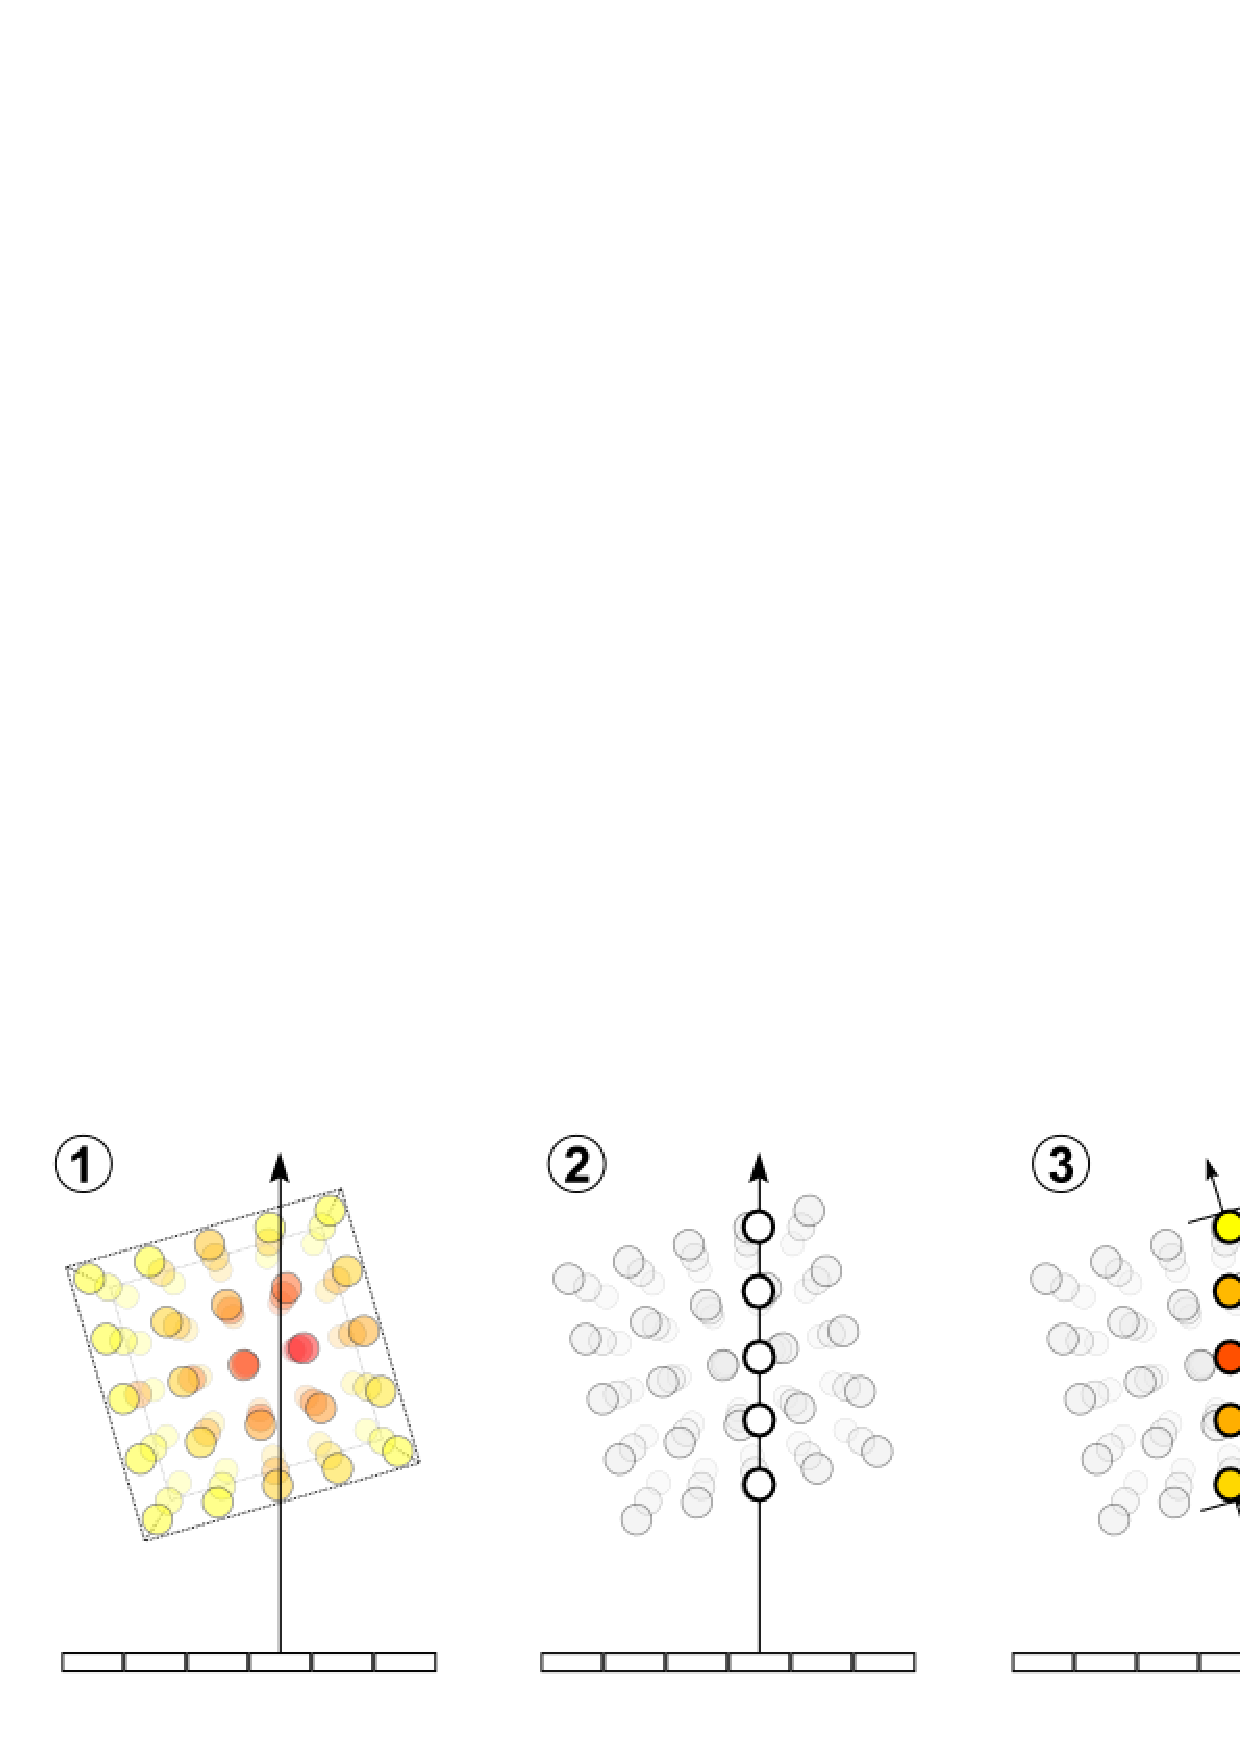
\includegraphics[width=0.4\textwidth]{img/Volumeraycasting.png}
}
\subfigure[Opacity transfer function]{
	\includegraphics[width=0.5\textwidth]{img/otf.png}
}
\caption{.}
\label{fig:vr}
\end{figure}

\subsection{Adaptive volume rendering}

Visibility driven visualization.

\section{Field simulations}\label{sec:field}

Small chapter about different simulation tools (See hos paper).
			
\endinput
